\documentclass[11pt, oneside]{article}
\usepackage{geometry}
\geometry{letterpaper}
\usepackage{graphicx}
\usepackage{amssymb}
\usepackage{amsmath}
\usepackage{tikz}
\usepackage{tikz-qtree}
\usepackage{url}
\usepackage[T1]{fontenc}

\title{SICP Exercise 3.27}
\author{Yuchong Pan}

\begin{document}
\maketitle

Initially, the environment structure created by \textbf{(define (memoize f) ...)} and by \textbf{(define memo-fib ...)}, where \textbf{table} is empty, is given as follows.

\begin{figure}[h!]
    \centering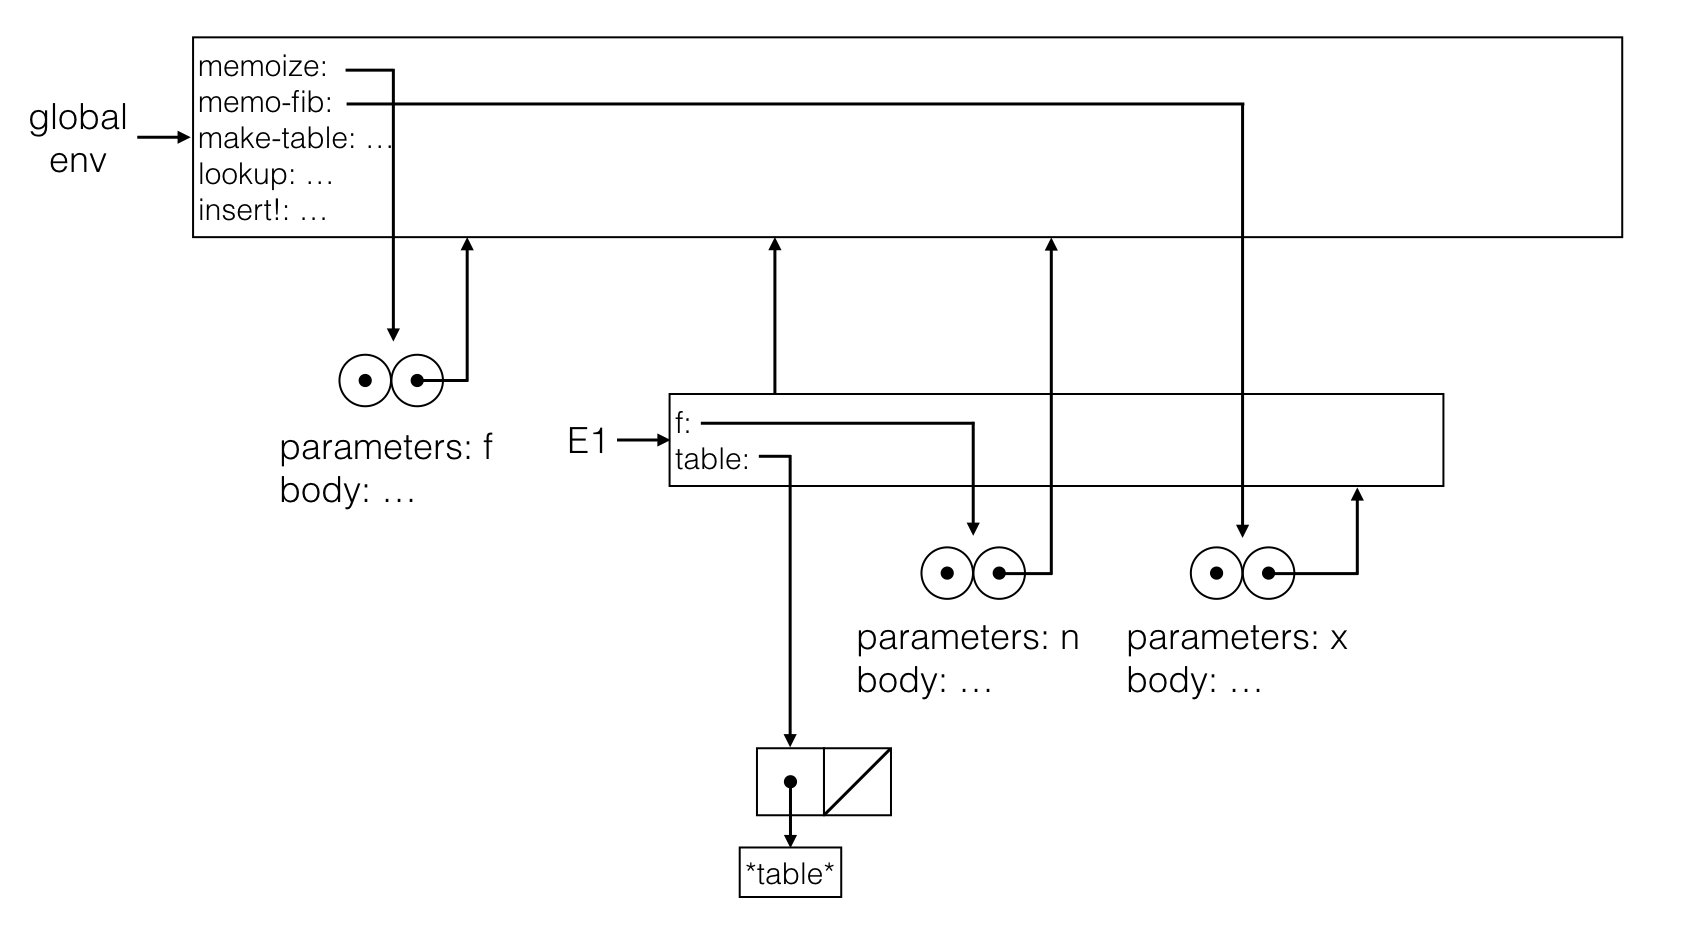
\includegraphics[width=15cm]{ex-3.27-1.png}
    \caption{Effect of \textbf{(define (memoize f) ...)} and of \textbf{(define memo-fib ...)}.}
\end{figure}

When \textbf{(memo-fib 3)} is called, a new environment is created, where \textbf{previously-computed-result} is computed to be \textbf{false} by \textbf{(lookup 3 table)}. Thus, \textbf{(f 3)} is called, and \textbf{(memo-fib 2)} and \textbf{(memo-fib 1)} is subsequently required.

Then, \textbf{(memo-fib 2)} is called. Similarly, \textbf{previously-computed-result} is computed to be \textbf{false}, and hence, \textbf{(f 2)} is called. The interpreter will subsequently compute \textbf{(memo-fib 1)} and \textbf{(memo-fib 0)}.

Thereafter, \textbf{(memo-fib 1)} is called, and \textbf{previously-computed-result} is still \textbf{false}, so \textbf{(f 1)} is called, where \textbf{(= n 1)} is a boundary condition and gives 1. Therefore, the record \textbf{(1, 1)} is added to \textbf{table}.

\begin{figure}[h!]
    \centering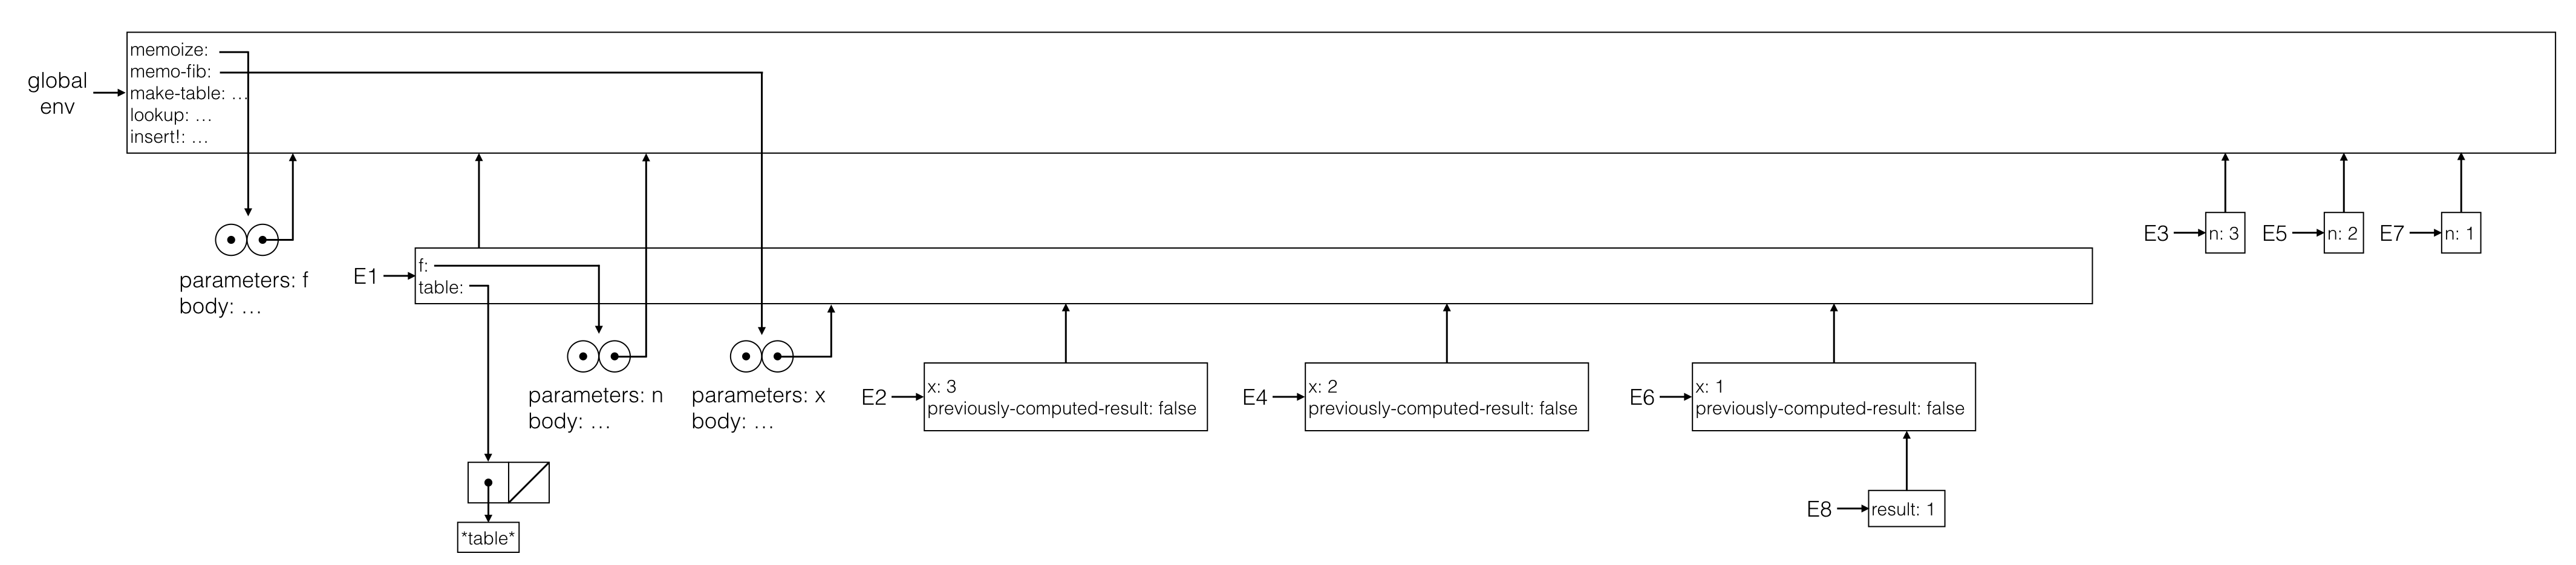
\includegraphics[width=15cm]{ex-3.27-2.png}
    \caption{Effect of \textbf{(memo-fib 3)}.}
\end{figure}

Likewise, \textbf{(memo-fib 0)} is called, where \textbf{previously-computed-result} is also \textbf{false}, so \textbf{(f 0)} is called, where \textbf{(= n 0)} is a boundary condition and gives 0. Therefore, the record \textbf{(0, 0)} is added to \textbf{table}.

\begin{figure}[h!]
    \centering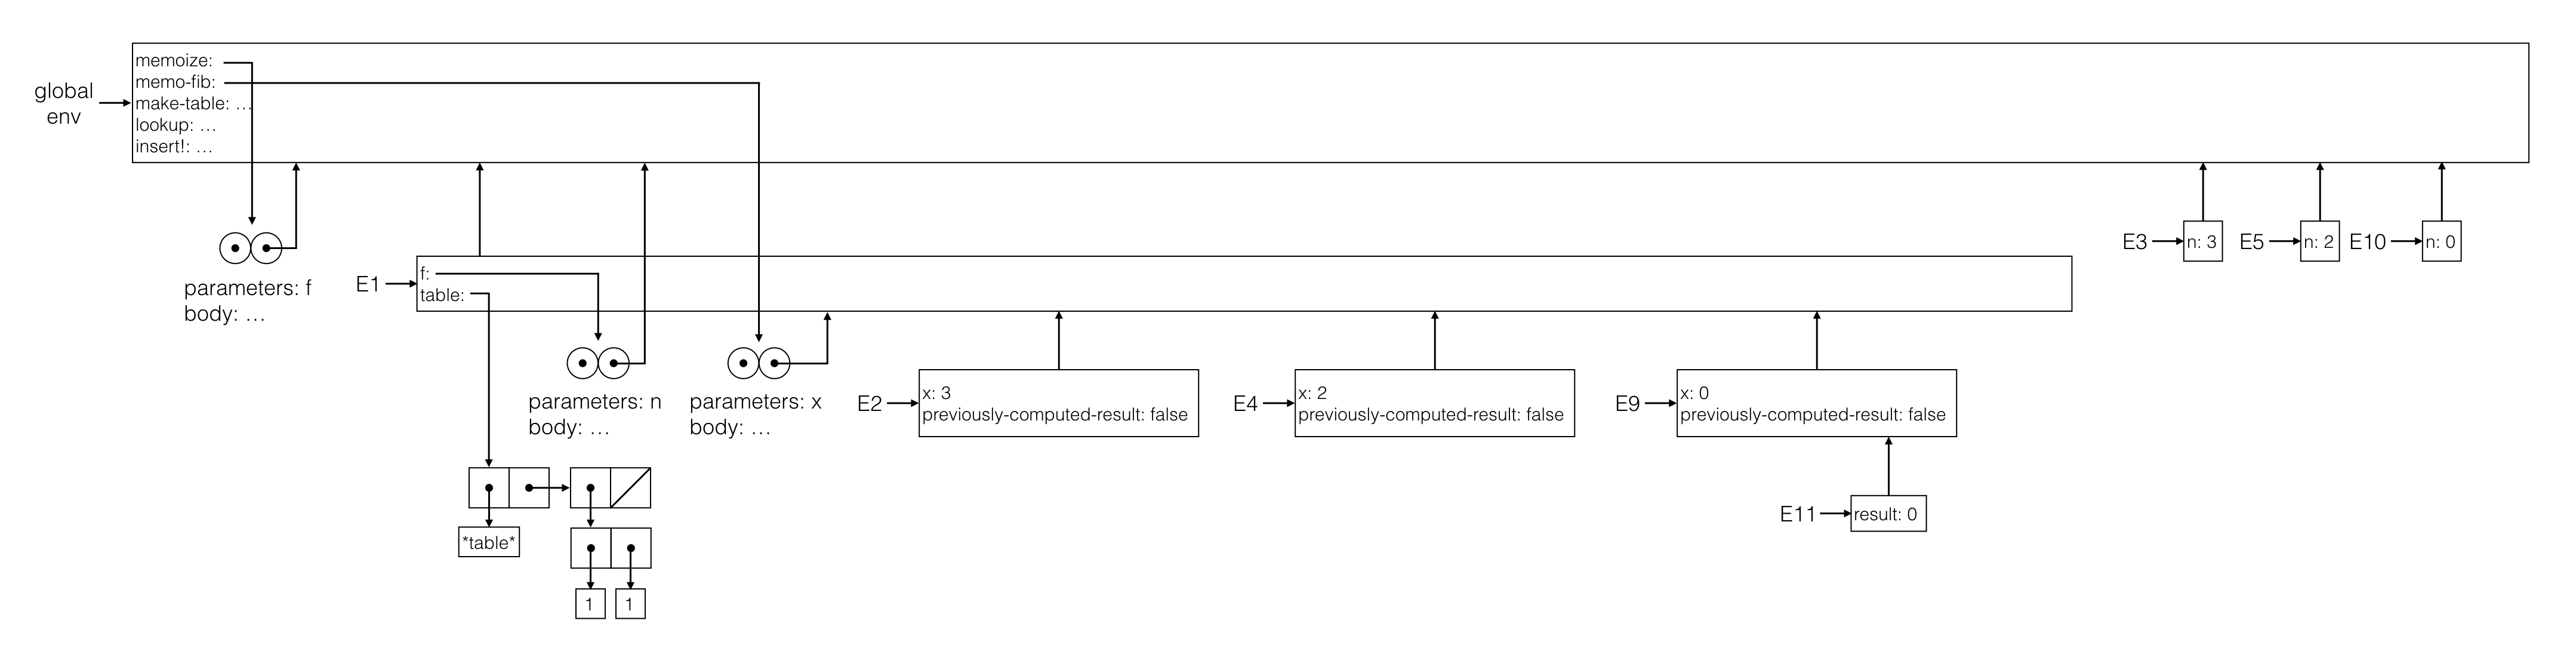
\includegraphics[width=15cm]{ex-3.27-3.png}
    \caption{Effect of \textbf{(memo-fib 3)}.}
\end{figure}

Having \textbf{(memo-fib 1)} and \textbf{(memo-fib 0)} computed, the result of \textbf{(memo-fib 2)} is the sum of the two computed results, i.e. 1. Thus, the record \textbf{(2, 1)} is added to \textbf{table}.

\begin{figure}[h!]
    \centering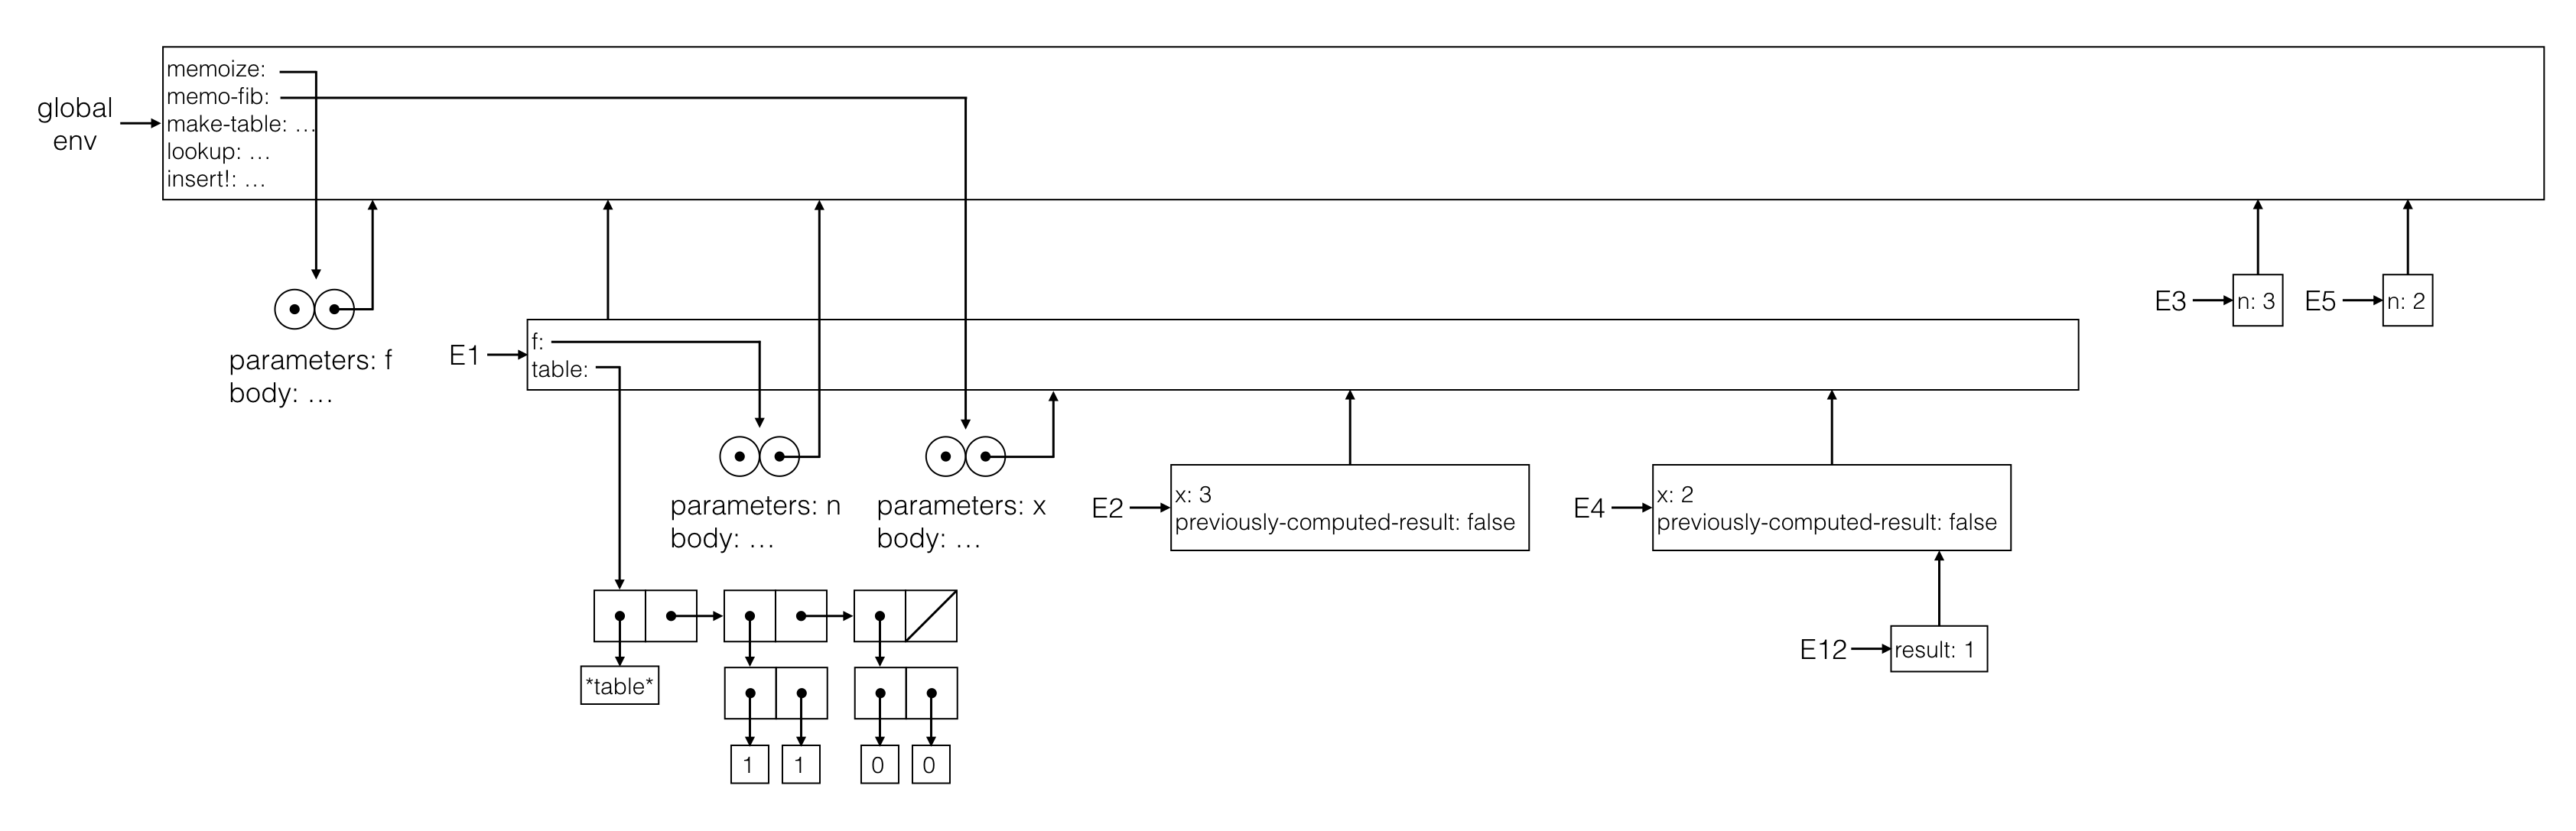
\includegraphics[width=15cm]{ex-3.27-4.png}
    \caption{Effect of \textbf{(memo-fib 3)}.}
\end{figure}

As mentioned above, \textbf{(f 3)} also requires \textbf{(memo-fib 1)}. At this point, the value 1 is searched in \textbf{table} with the key 1. Hence, the result of \textbf{(memo-fib 1)} is 1, and the result of \textbf{(f 3)} is the sum of \textbf{(memo-fib 2)} and \textbf{(memo-fib 1)}, which gives 2. The record \textbf{(3, 2)} is added to \textbf{table}. Therefore, the computation of \textbf{(memo-fib 3)} gives 2.

\begin{figure}[h!]
    \centering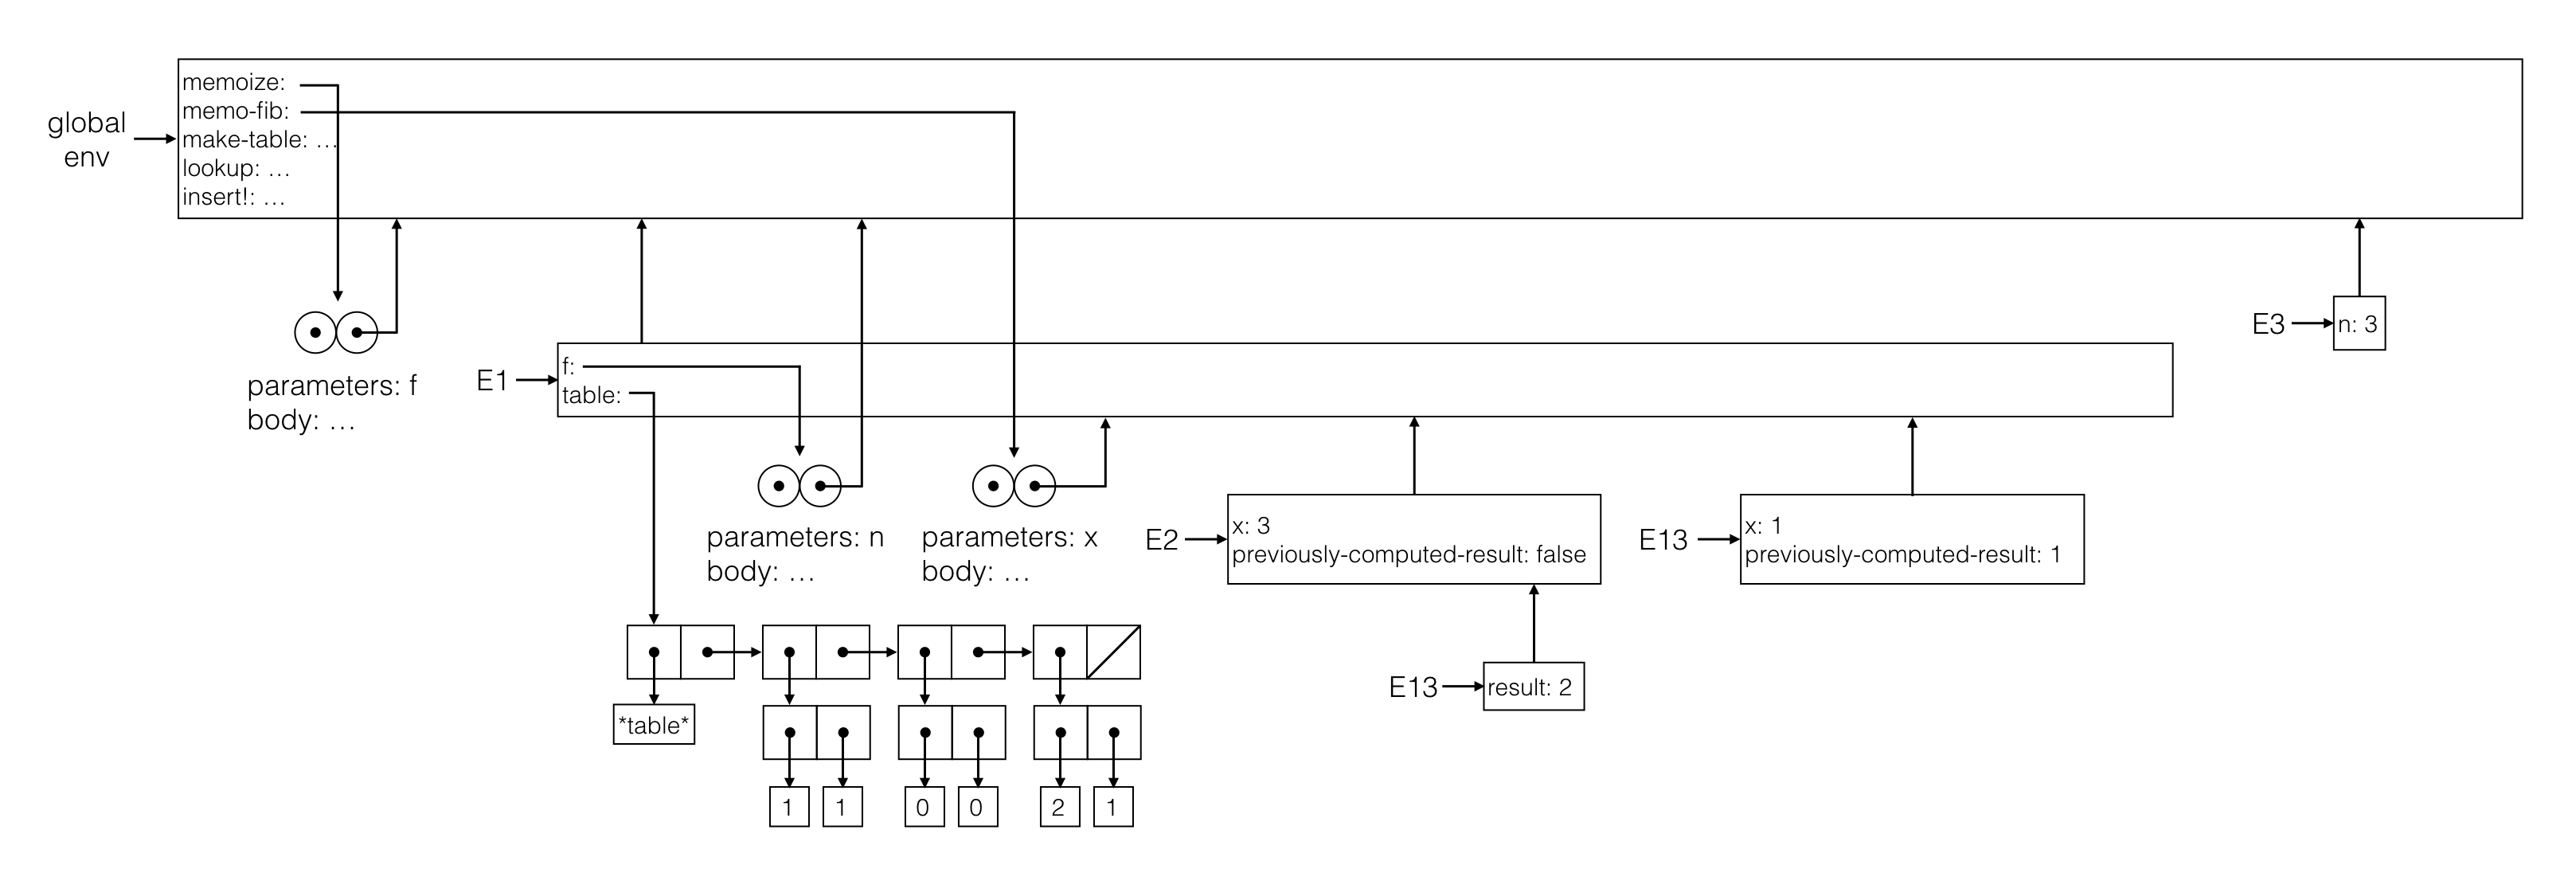
\includegraphics[width=15cm]{ex-3.27-5.png}
    \caption{Effect of \textbf{(memo-fib 3)}.}
\end{figure}

\begin{figure}[h!]
    \centering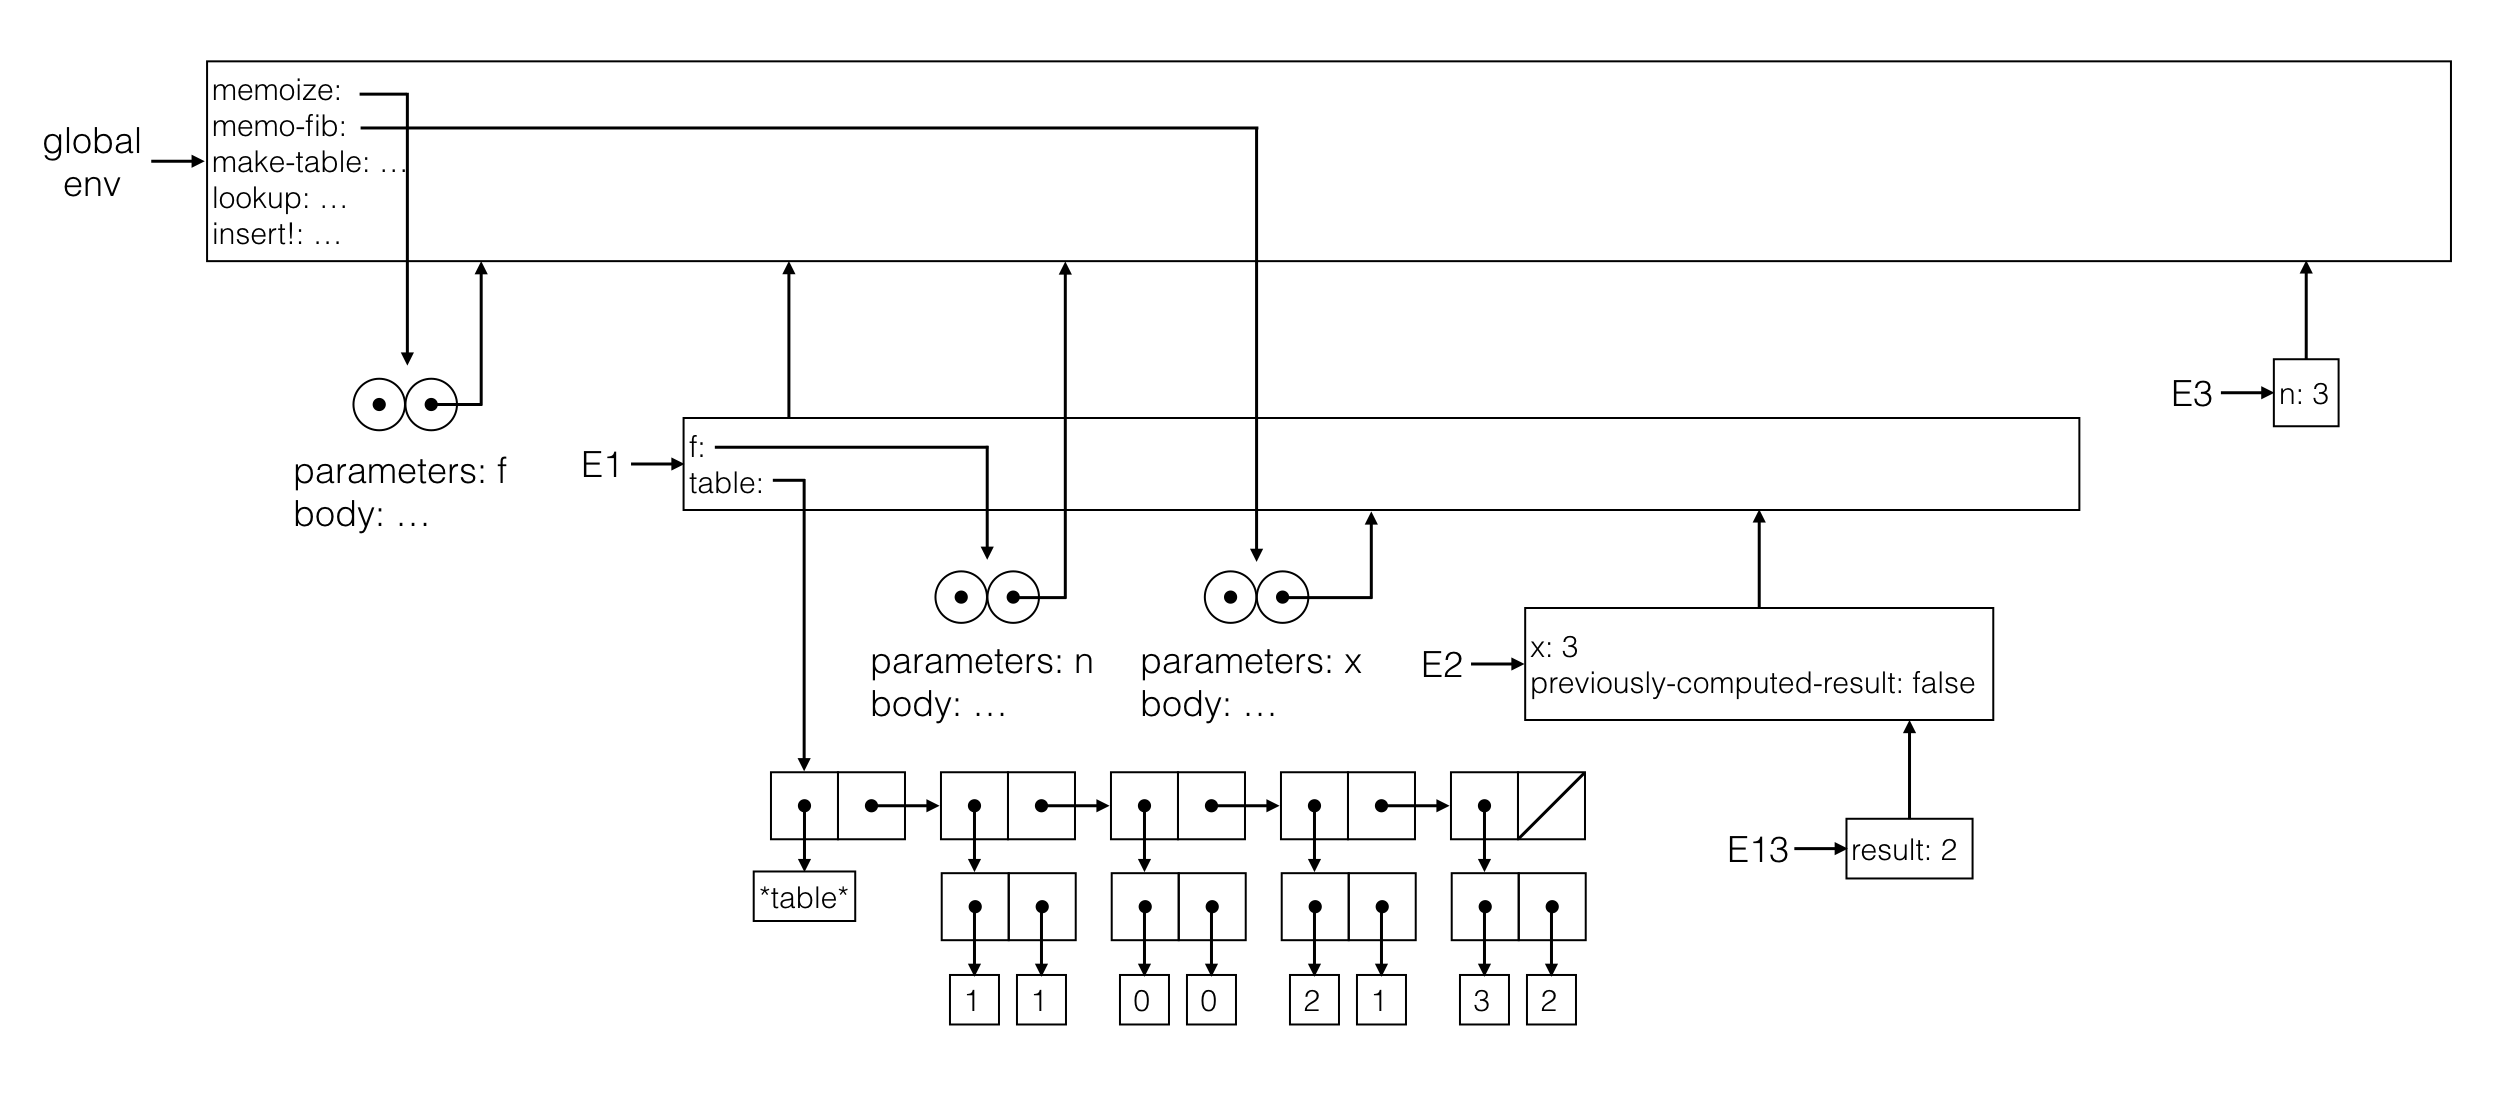
\includegraphics[width=15cm]{ex-3.27-6.png}
    \caption{Effect of \textbf{(memo-fib 3)}.}
\end{figure}

Since \textbf{table} is maintain in which values of previous calls are stored using as keys the arguments that produces the values, \textbf{(memo-fib $i$)} where $1 \leq i \leq n$ will be called at most once when \textbf{(memo-fib $n$)} computes the $n$th Fibonacci number. Therefore, the number of steps required by the computation of \textbf{(memo-fib $n$)} is proportional to $n$; i.e., the number of steps grows as $\Theta(n)$.

If \textbf{memo-fib} is simply defined to be \textbf{(memoize fib)}, the scheme would not work. If the key $n$ is not found in \textbf{table} when \textbf{(memo-fib $n$)} is called and when $n > 1$, then the interpreter will subsequently call \textbf{(fib (- n 1))} and \textbf{(fib (- n 2))}, which cannot use memoization any longer and will perform as the original \textbf{fib}. Thus, the number of steps required by \textbf{(memo-fib $n$)} will grows as $\Theta(Fib(n))$ rather than $\Theta(n)$.

\end{document}
